\chapter{Launch and manage instances}\label{cha:launch-manage-inst}
Instances are virtual machines that run inside the cloud. You can launch
an \gls{instance} from the following sources:

\begin{itemize}
\item Images uploaded to the Image service.

  \strong{Note:} Because images are read-only, any changes made while
  the instance is running will be lost when the instance is deleted,
  unless you choose to create a persistent volume for your instance
  when you launch it.  Using a volume, the VM's state is saved, even
  when the current instance is deleted.
\item Images which you previously copied to a persistent volume. The
  instance launches from the volume.
\item Instance snapshots.
\end{itemize}

\section{Launch an instance}\label{launch-an-instance}
\begin{enumerate}
\item Open the Compute tab and select the Instances category.

  The dashboard shows the list of existing instances with their name,
  IP addresses, flavor, status, power state, \ldots
\item Click \strong{Launch Instance}.
\item In the Launch Instance dialog box, specify the following values:

  \begin{center}
    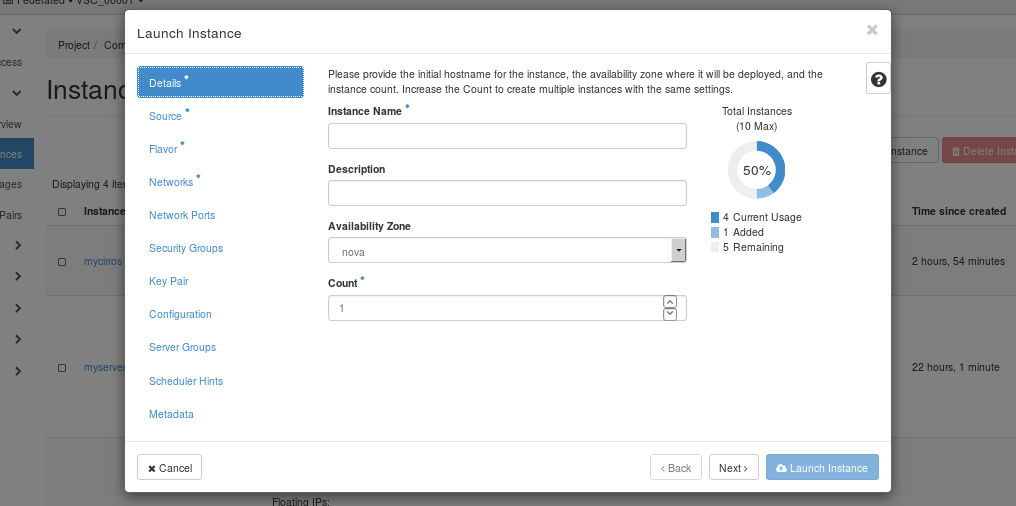
\includegraphics[scale=0.5]{img/tab-compute-instances-launch.png}
  \end{center}
  
  \begin{description}
  \item[Details] tab
    \begin{description}
    \item[Instance Name] Assign a name to the virtual machine.

      \strong{Note:} The name you assign here becomes the initial host
      name of the server. If the name is longer than 63 characters,
      the Compute service truncates it automatically to ensure dnsmasq
      works correctly.

      After the server is built, if you change the server name in the
      API or change the host name directly, the names are not updated
      in the dashboard.

      Server names are not guaranteed to be unique when created so you
      could have two instances with the same host name.

    \item[Description] You can assign a brief description of the
      virtual machine.
    \item[Availability Zone] By default, this value is set to the
      availability zone given by the cloud provider (for example,
      \strong{us-west} or \strong{apac-south}).  For some cases, it
      could be \strong{nova}.
    \item[Count] To launch multiple instances, enter a value greater
      than \strong{1}. The default is \strong{1}.
    \end{description}

    \begin{center}
      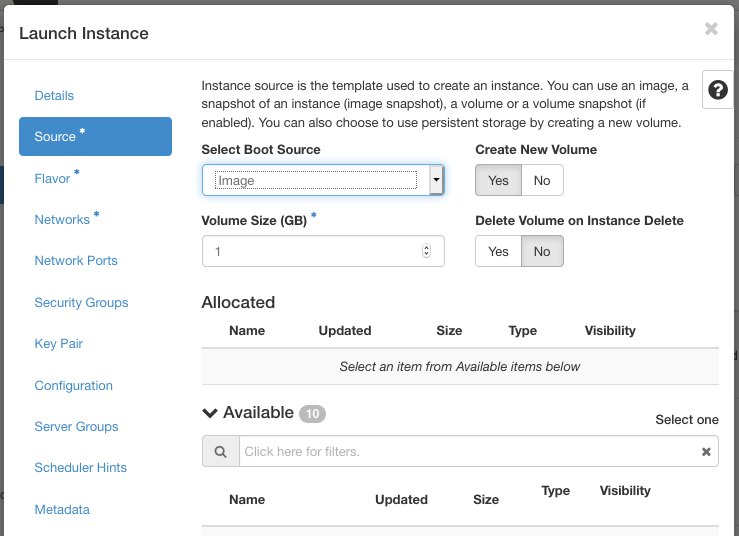
\includegraphics[width=0.7\textwidth]{img/launch_instance_source}
    \end{center}
  \item[Source] tab
  \begin{description}
  \item[Select Boot Source] Your options are:
    \begin{description}
    \item[Image]
    \item[Image snapshot]
    \item[Volume]
    \item[Volume snapshot]
    \end{description}
    Depending on the type of boot source, the list of available items
    changes.

  \item[Create New Volume] If you enable this option when launching
    from an image or instance snapshot, the image or snapshot will be
    copied to a volume.  This way, the state of your instance persists
    after shutdown and reboot.
  \end{description}

\item[Flavor] tab. Specify the size of the instance to launch.

  \strong{Note:} The flavor is selected based on the size of the image
  selected for launching an instance. For example, while creating an
  image, if you have entered the value in the Minimum RAM (MB) field
  as 2048, then on selecting the image, the default flavor is
  \strong{m1.small}.  If a `!' warning sign is displayed next to a
  resource for one of the flavors, that means that this flavor would
  exceed the project's quota for that resource, and therefore is not
  available.

\item[Networks] tab. Add one or more networks to the instance.

\item[Network Ports] tab. Activate the ports that you want to assign to
  the instance.
\item[Security Groups] tab. Activate the security groups that you want
  to assign to the instance.

  Security groups are a kind of cloud firewall that define which
  incoming network traffic is forwarded to instances.  See section
  \ref{cha:conf-access-secur} on page ~\pageref{sec:security-groups}
  for more information.

  The default security group is assigned to the instance
  automatically.
\item[Key Pair] tab. Specify a key pair.

  If the image uses a static root password or a static key set
  (neither is recommended), you do not need to provide a key pair to
  launch the instance.
\item[Configuration] tab. Specify a customization script that runs
  after your instance launches.

\item[Server Groups] tab.

\item[Scheduler Hints] tab.

\item[Metadata] tab. Add Metadata items to your instance.
\end{description}

\item Click \strong{Launch Instance}.
\end{enumerate}

The instance starts on a compute node in the cloud.

\strong{Note:} If you did not provide a key pair, security groups, or
rules, users can access the instance only from inside the cloud
through VNC. Even pinging the instance is not possible without an ICMP
rule configured.

You can also launch an instance from the Images or Volumes category when
you launch an instance from an image or a volume respectively.

When you launch an instance from an image, OpenStack creates a local
copy of the image on the compute node where the instance starts.

For details on creating images, see
\href{https://docs.openstack.org/image-guide/create-images-manually.html}{\emph{Creating
images manually}} in the \emph{OpenStack Virtual Machine Image Guide}.

\section{Connect to an instance using SSH}\label{connect-to-your-instance-using-ssh}
Before you can connect to an instance using SSH, you must set up a
floating IP for it, as discussed in section~\ref{sec:floating-ip}.
Recall that only ports 50000 to 60000 of the floating IP's can be
directly reached from outside the UGent network.

\strong{Note:} When you try to connect to a new instance using a port
that was previously forwarded to a different instance --- either due
to a change in the port forwarding configuration, or because an old
instance was deleted and replaced --- your SSH client will show an
error message because the ``host key'' of the new instance doesn't
match the known previous key.  Section \nameref{sec:host-keys}
explains how to handle such errors.

\strong{Note:} If you want to access ports outside the public range,
you'll need to connect to the UGent login node
\lstinline{login.hpc.ugent.be} first, and hop to your instance from
there.  To make this work without storing the required private key for
the instance in your VSC storage space, you need to set up an SSH
agent with key forwarding locally, i.e.\ on the machine where you
store the private key of an authorized keypair for the instance.
Section 2.1.4 of the HPC introduction explains how to set this up
(\href{https://hpcugent.github.io/vsc\_user\_docs}{hpcugent.github.io/vsc\_user\_docs}).

\begin{enumerate}
  \setcounter{enumi}{-1}
\item (\emph{Only if using a port blocked by the UGent firewall, see
    the note above:}) Use your VSC account to connect to the UGent login
  node, using the \lstinline{ssh -A} option to enable agent
  forwarding:

  \begin{prompt}
    %\shellcmd{ssh -A vsc12345@login.hpc.ugent.be}
  \end{prompt}

\item Copy the address of the floating IP where your instance can be
  reached.  In our example, the address is 193.190.85.40.

\item Connect to the instance.  Use OpenSSH's \lstinline{-p} option to
  specify the port where the instance's SSH server can be reached,
  e.g. for port 50022:

  \begin{prompt}
    %\shellcmd{ssh -p 50022 ubuntu@193.190.85.40}
  \end{prompt}

  When you run the above command, your SSH client may display warnings
  or error messages.  The section \nameref{sec:host-keys}
  explains the meaning of these messages and how you should deal with
  them.

  \strong{Note:} The images we provide do not allow SSH logins for the
  root user.  There is a default user instead, who can get
  administrative privileges using \lstinline{sudo}.  In our example,
  we have used the username \lstinline{ubuntu} for Ubuntu images.
  Attempting to log in as root will return an error message with the
  proper user name.
\end{enumerate}

\subsection*{Host keys}\label{sec:host-keys}
When connecting to instances using SSH, you will sometimes see
warnings or errors related to ``host keys''.  This section briefly
explains the meaning of those errors, and how to deal with them.

When you try to connect to an instance, you use the private key of
your SSH keypair to prove your identity to that instance.  If you do
not have access to the right secret key, you can not prove your
identity, at which point the your instance's SSH server will deny
access.  In the same way, the server must prove its own identity to
you, using its own keypair or ``host key''.  Without such a
verification procedure, third parties on the network between you and
the instance could perform a so-called man-in-the-middle-attack, where
they intercept the communication between you and the server you want
to reach and steal valuable information.

To prevent such man-in-the-middle attacks, the SSH client on your
system keeps a list of known host keys for every IP address you have
connected to, and verifies the host key the next time you try to
connect to that address.  If all goes well, this check is silently
performed in the background, but there are a number of situations
where the check fails.  In this case, you have to look up the host key
of your instance using the OpenStack dashboard to verify that the
connection is secure.

\subsubsection*{Looking up an instance's host
  key}\label{sec:look-up-hostkey}
In order to verify a host key, it suffices to compare the key's
fingerprint, a short alphanumerical sequence computed from the keys
content.  You can use the Dashboard to look up the host key
fingerprint for an instance as follows:
\begin{enumerate}
\item Open the Compute tab and select the Instances category.
\item Click on the name of the instance you want to connect to.
\item Click \strong{Log}
  \begin{center}
    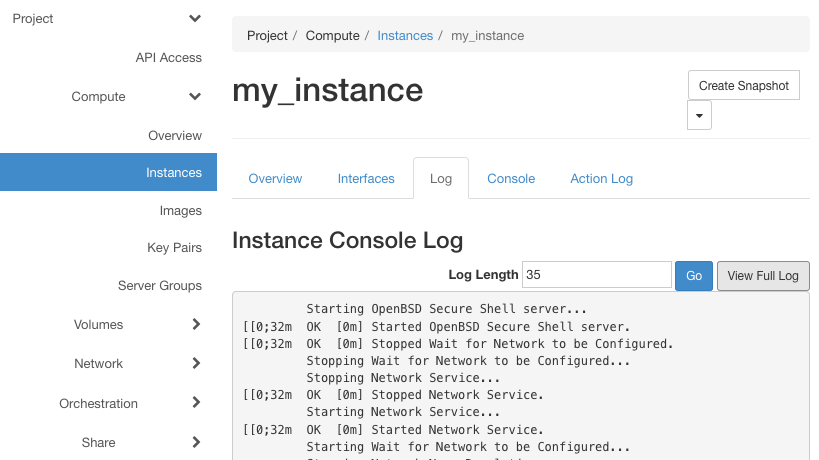
\includegraphics[width=0.8\textwidth]{img/instance_log}
  \end{center}

\item Click \strong{View Full Log}.  You are taken to a new page with a long text listing.
\item Search for the words \lstinline{-----BEGIN SSH HOST KEY FINGERPRINTS-----} to find the log file section containing the host key fingerprints, for example:
\begin{code}{}
<14>Jun  6 09:57:01 ec2: #############################################################
<14>Jun  6 09:57:01 ec2: -----BEGIN SSH HOST KEY FINGERPRINTS-----
<14>Jun  6 09:57:01 ec2: 1024 SHA256:gCa0hZAaOnpzxYM5WnAZINuZTI5NAoqd41U/dtxeGKE root@my-instance (DSA)
<14>Jun  6 09:57:01 ec2: 256 SHA256:nyujUIF37c674FPSkDdz0xgAU6S39UWbmMzBPmdmCmg root@my-instance (ECDSA)
<14>Jun  6 09:57:01 ec2: 256 SHA256:Mcznquek1A3BFz6KEXSxsivpdkX1mY3LnymEA7C8Xxg root@my-instance (ED25519)
<14>Jun  6 09:57:01 ec2: 2048 SHA256:4DagYc9cZvANkSjbTL0pB+3ULqHg09zW4E8wvDrB4Do root@my-instance (RSA)
<14>Jun  6 09:57:01 ec2: -----END SSH HOST KEY FINGERPRINTS-----
<14>Jun  6 09:57:01 ec2: #############################################################
\end{code}
\end{enumerate}

In this example, the fingerprints are character sequences starting
with ``SHA256'', such as the ECDSA key fingerprint
\lstinline{SHA256:nyujUIF37c674FPSkDdz0xgAU6S39UWbmMzBPmdmCmg}.  The
following sections describe the most common cases where you'll need
these fingerprints.

\subsubsection*{Connecting for the first time}\label{sec:conn-first-time}
The first time you connect to a new ip address:port combination, your SSH client does not know the host key for this address, and therefore it can't verify the identity of the server.  When using OpenSSH, the warning looks as follows (again using address 193.190.85.40 and port 50022 as an example):

\begin{prompt}
The authenticity of host '[193.190.85.40]:50022 ([193.190.85.40]:50022)'
can't be established.
ECDSA key fingerprint is SHA256:nyujUIF37c674FPSkDdz0xgAU6S39UWbmMzBPmdmCmg.
Are you sure you want to continue connecting (yes/no)?
\end{prompt}

Verify the fingerprint in order to make sure that it is safe to
proceed:

\begin{enumerate}
\item Look up the fingerprint of the instance you want to access,
  according to the procedure described in the section
  \nameref{sec:look-up-hostkey}.
\item Verify that the fingerprint you find in the Dashboard matches
  the fingerprint shown in the warning message.

  In this example, we see that the ECDSA key fingerprint reported by
  the SSH client matches the fingerprint of our instance from the
  previous section, namely

  \lstinline{SHA256:nyujUIF37c674FPSkDdz0xgAU6S39UWbmMzBPmdmCmg}.

\item If the fingerprints are identical, type ``yes'' to log in.
  \strong{If the fingerprints do not match, type ``no'', and contact
    \cloudinfo.}
\end{enumerate}

\subsubsection{New instance at a known address}
Another case where the host key verification fails, is when you try to access a new instance at an IP address and port previously used by another instance.  This can happen if you modify your port forwarding configuration, or if a running instance connected to a certain port is deleted and replaced by a new one.  In this case, OpenSSH will show a warning such as this:

\begin{prompt}
@@@@@@@@@@@@@@@@@@@@@@@@@@@@@@@@@@@@@@@@@@@@@@@@@@@@@@@@@@@
@    WARNING: REMOTE HOST IDENTIFICATION HAS CHANGED!     @
@@@@@@@@@@@@@@@@@@@@@@@@@@@@@@@@@@@@@@@@@@@@@@@@@@@@@@@@@@@
IT IS POSSIBLE THAT SOMEONE IS DOING SOMETHING NASTY!
Someone could be eavesdropping on you right now (man-in-the-middle attack)!
It is also possible that a host key has just been changed.
The fingerprint for the ECDSA key sent by the remote host is
SHA256:hI2HcqFxsCKwEauq2QvBmgDN4nCPjllaRsYoCb7tJQw.
Please contact your system administrator.
Add correct host key in [...]/.ssh/known_hosts to get rid of this message.
Offending ECDSA key in [...]/.ssh/known_hosts:57
ECDSA host key for [193.190.85.40]:50322 has changed and you have requested strict checking.
Host key verification failed.
\end{prompt}

The file \lstinline{known_hosts} in your OpenSSH configuration
directory contains a list of all hosts you have previously connected
to, together with their host keys.  The warning above tells you that
the server you are connecting to is not using the same key anymore.
In this case, you should take the following steps:
\begin{enumerate}
\item Look up the fingerprint of the instance you want to access,
  according to the procedure described in the section
  \nameref{sec:look-up-hostkey}.
\item Verify that the fingerprint you find in the Dashboard matches
  the fingerprint shown in the warning message.
\item If the fingerprint matches, the new key is legitimate. Remove
  the previous known key from the \lstinline{known_hosts} file as
  follows (still using address 193.190.85.40 and port number 50322 as
  an example):

  \begin{prompt}
    % \shellcmd{ssh-keygen -R [193.190.85.40]:50322}%\end{prompt}

    This command causes OpenSSH to forget the previous key.  On your
    next attempt to connect to that address, OpenSSH will treat it as
    a new host and ask you to verify the fingerprint as described in
    section \nameref{sec:conn-first-time}.

  \strong{If the fingerprint does not match, do not attempt to connect, and contact \cloudinfo.}
\end{enumerate}

\section{Track usage for instances}\label{track-usage-for-instances}

You can track usage for instances for each project. You can track costs
per month by showing meters like number of vCPUs, disks, RAM, and uptime
for all your instances.

\begin{enumerate}
\item Open the Compute tab and select the Overview category.
\item To query the instance usage for a period of time, select a time
  range and click \strong{Submit}.
\item To download a summary, click \strong{Download CSV Summary}.
\end{enumerate}

\section{Create an instance snapshot}\label{create-an-instance-snapshot}

\begin{enumerate}
\item Open the Compute tab and select the Instances category.
\item Select the instance from which to create a snapshot.
\item In the actions column, click \strong{Create Snapshot}.
\item In the Create Snapshot dialog box, enter a name for the snapshot, and
  click \strong{Create Snapshot}.
\end{enumerate}

The Images category shows the instance snapshot.

To launch an instance from the snapshot, select the snapshot and click
Launch. Proceed with launching an instance.

\section{Manage an instance}\label{manage-an-instance}

\begin{enumerate}
\item Open the Compute tab and select the Instances category.
\item Select an instance.
\item In the menu list in the actions column, select the state.

  You can resize or rebuild an instance. You can also choose to view
  the instance console log, edit instance or the security
  groups. Depending on the current state of the instance, you can
  pause, resume, suspend, soft or hard reboot, or terminate it.
\end{enumerate}

\subsection*{Difference between \emph{suspend}, \emph{pause}, \emph{shelve}, \emph{shut off}, \emph{delete}}\label{server-power-down-states}

\begin{description}
\item[Pause] Stores the state of the VM in the (RAM) memory.
\item[Suspend] Stores the state of the VM on the disk, all memory is
  written to disk, and the server is stopped.
\item[Shut off] The server is powered down by the user, either through
  the OpenStack Compute API, or from within the server by issuing a
  \emph{shutdown -h} command. In this state the user retains all
  computational resources associated with the VM. The instance can be
  later restarted.
\item[Shelve] Shelving stops the instance and takes a snapshot of
  it. Then depending on the value of the \emph{shelved\_offload\_time}
  config option, the instance is either deleted from the hypervisor
  (0), never deleted (-1), or deleted after some period of time (>
  0). Shelve preserves all associated data and VM resources but does
  not retain anything in memory.
\item[Delete] The VM is deleted and removed from \gls{OpenStack}
  together with any associated processes and resources.  However, for
  instances backed by a persistent volume, this volume is not deleted.
  When such an instance is deleted, you can restore it by launching a
  new instance from the volume, or delete the volume as well (see
  section \ref{delete-a-volume}).
\end{description}

For more details see the OpenStack documentation on \href{https://docs.openstack.org/nova/\osversion/reference/vm-states.html}{\emph{Virtual Machine States and Transitions}} and \href{https://developer.openstack.org/api-guide/compute/server_concepts.html}{\emph{Server concepts}}.

%%% Local Variables:
%%% mode: latex
%%% TeX-master: "intro-Cloud"
%%% End:
